%%%%%%%%%%%%%%%%%%%%%%%%%%%%%%%%%%%%%%%%%%%%%%%%%%%%%%%%%%%%%%%%%
\chapter{INTRODUCTION TO MACHINE LEARNING}\label{ch:CH4}
%%%%%%%%%%%%%%%%%%%%%%%%%%%%%%%%%%%%%%%%%%%%%%%%%%%%%%%%%%%%%%%%%

In this chapter, we start with the basics of machine learning. Then we mention cross-validation approach, which is a model evaluation technique, and the regularization concept. Finally, we end the section with the ML algorithms used in the thesis.

\begin{figure}[h]
	\centering
	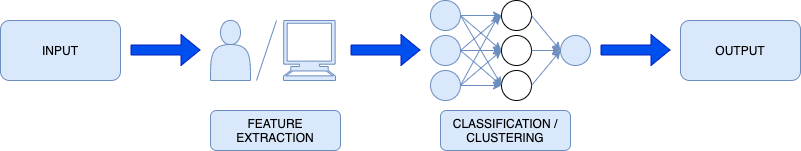
\includegraphics[width=\linewidth]{fig/basic_ml.png}
	\vspace*{2mm}
	\caption{Sample Machine Learning Road Map.}
	\label{basic_ml}
\end{figure}

\section{The Basics of Machine Learning (ML)}

The goal of machine learning (Ml) is to learn from available data or experiences to solve a given problem. The pipeline may be listed as:

\begin{itemize}
    \item defining the problem to solve,
    \item collecting the data for training and testing,
    \item designing or extracting the features describing data,
    \item training the model to tune the parameters by experiments and optimization on the appropriate loss function, and
    \item testing the model to evaluate the performance of trained model on unseen test data.
\end{itemize}

The majority of the problems in ML are fall into supervised and unsupervised learning approaches.

\begin{figure}[h]
	\centering
	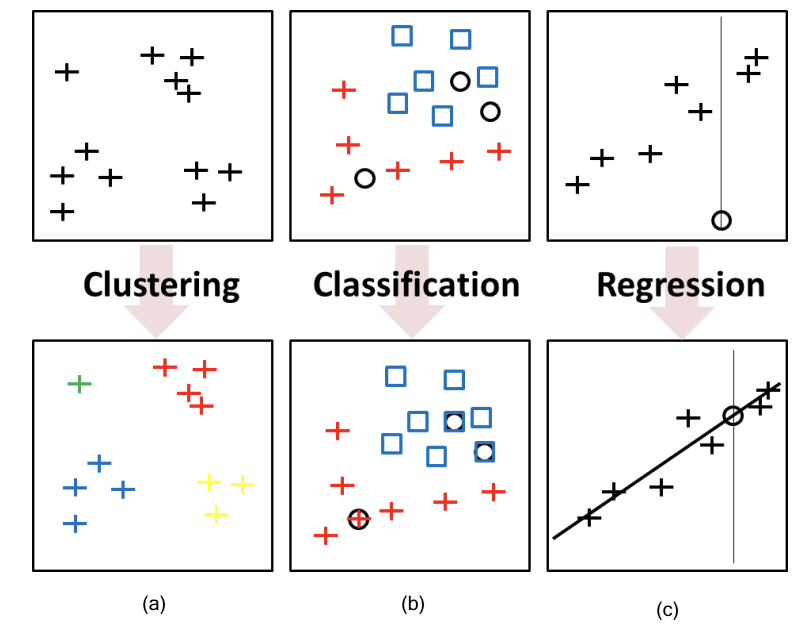
\includegraphics[width=.8\linewidth]{fig/clustering_classification_regression.png}
	\caption{(a) Clustering Problem, (b) Classification Problem, and (c) Regression Problem \cite{parallel_linear_algebra}.}
	\label{clustering_classification_regression}
\end{figure}

\subsection{Supervised Learning}

Supervised learning is a ML method that establishes a relationship between the each attribute of data feature map and its target value. Estimating the output value for each new datum is the main goal. All true target values are known during training and testing. These known true values are used to construct the trained model, and to evaluate the testing performance. Regression and classification problems are solved by supervised learning.

The task in this thesis includes dataset in that each datum has its true label value. Thus, all ML models used in this thesis are from supervised learning algorithms.

\subsection{Unsupervised Learning}

The problems having data with unknown true values are solved by unsupervised learning. While there are hard or impossible to labeling data sets, some data sets can be deliberately left unlabeled since it requires too much time, expert people and special devices to label. Clustering tasks are constructed on these kind of data sets and solved by unsupervised learning.

\section{Cross-Validation (CV)}

As in deep learning, overfitting and underfitting are also big troubles in machine leaning. Cross-validation (CV) methods can be used to overcome these problems. In the CV method, all data is divided into train and test sets. Here, it should not be forgotten that the train and test sets must be strictly separated from each other, and any sample on test set should not be seen during training process.

\begin{figure}[h]
	\centering
	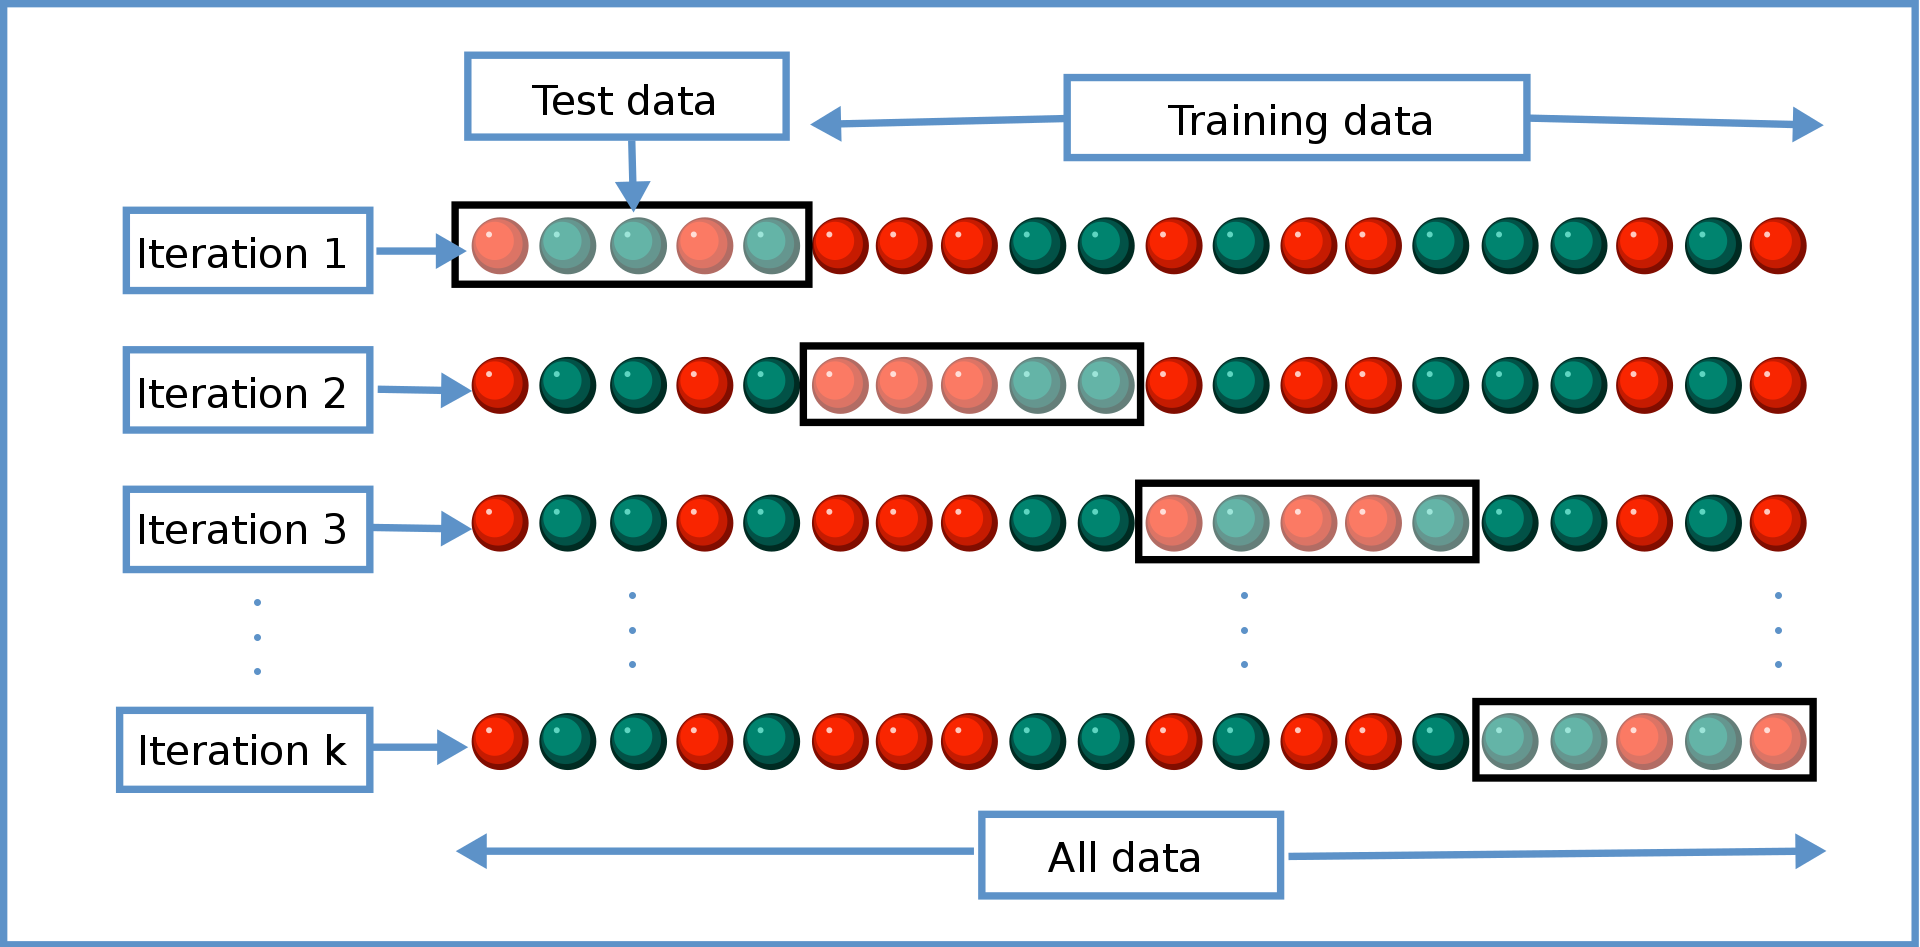
\includegraphics[width=.8\linewidth]{fig/k_fold_cv.png}
	\vspace*{2mm}
	\captionfootnotemark{K-Fold Cross-Validation.}
	\label{k_fold_cv}
\end{figure}
\footnotetext{Retrieved from: \hyperrefurl{https://towardsdatascience.com/cross-validation-c4fae714f1c5} on April 10, 2021.}

\subsection{K-Fold CV}

On K-Fold CV, K is the hyper-parameter to tune that defines the number of folds during partitioning. The choice of K must be greater than 1 and less than the number of data. All data is divided into K folds of the same (if possible) or different sizes. The folds are enumerated from 1 to K. Here, the model is evaluated and tested $(K-1)$ times. On each iteration $i$, where $i$ is an integer from 1 to K, the $i^{th}$ fold is chosen as the test set and rest as the train set, and model forgets what it learned previously and starts from zero. Otherwise, the test data on the $(i+1)^{th}$ iteration takes place in the train set on the $i^{th}$ iteration and is learned by the model.

\subsection{Leave-One-Out (LOO)}

If the K of K-Fold CV is chosen as the number of data, say N, it is a special case of CV and called as leave-one-out (LOO) method. As a convenience, all data are enumerated from 1 to N. Thus, model is evaluated and tested for N times. On each iteration $i$, where $i$ is an integer from 1 to N, the $i^{th}$ datum is chosen as the test sample and rest as the train set, and model forgets what it learned previously and starts from zero. Otherwise, the test sample on the current iteration takes place in the train set on the previous iteration and is learned by the model.

Briefly, LOO is the K-Fold CV where the number of folds is chosen as the number of data.

\section{Regularization}
\label{sec:CH5_regularization}

As discussed in Section~\ref{sec:CH3_the_basics_of_optimization}, the training process includes the optimization of corresponding loss function in machine learning. To minimize the loss and obtain the more optimized results, the regularization term is applied to the objective loss function. In general, the regularized loss function for supervised learning can be motivated as:

\be
\label{eq:general_regularized_loss}
\sum_{(x^{i}, y^{i} \in D)} \Big(\frac{Error(f_{w}(x^i), y^{i})}{n}\Big) + \lambda R(f_{w}), 
\ee

where $n$ is the number of training samples, $D$ is the training feature set with $x^{i}$ as training input and $y^{i}$ as the corresponding target output, $f_{w}$ is the mapping function between feature map and target values, $\lambda$ is a real number hyper-parameter greater than or equal to zero controlling the effect of regularization term, and $R$ is the regularization term. 

Notice that, if $\lambda$ is chosen as too high, the regularizer drowns out the loss function; and, if $\lambda$ is chosen as zero, there is no regularization. $\lambda$ is usually chosen between $0$ and $0.1$; however, it must be tuned for the corresponding task.

In addition, the regularization term $R$ has a constraint such that $R(f_{w}) \leq \mu$ for an appropriate real valued constant $\mu$.

The regularization is also called as penalty to the objective function. In this section, we focus on LASSO penalty and Ridge regression concepts which are used in this thesis.

\subsection{L1 Regularization (LASSO)}

L1 regularization term, which is known as LASSO, only penalizes the high coefficients. The LASSO penalty is in the form of:

\be
\label{eq:lasso_term}
\lambda \norm{w}_{1},
\ee

where w is the weight coefficients to optimize, and $\norm{.}_{1}$ is the L1 norm such that:

\be
\label{eq:l1_norm}
\norm{x} = \sum_{i=1}^{p} | x_{i} |,
\ee

for a vector $x$ in the size of $p$.

LASSO penalty may produce non-unique solutions \cite{lasso_penalty}.

\subsection{L2 Regularization (Ridge)}

L2 regularization term is known as Ridge regression. The penalty term in Ridge regression is in the form of:

\be
\label{eq:ridge_term}
\lambda \norm{w}_{2}^{2},
\ee

where w is the weight coefficients to optimize, and $\norm{.}_{2}^{2}$ is the squared L2 norm such that:

\be
\label{eq:l2_norm}
\norm{x}_{2}^{2} = \sum_{i=1}^{p} x_{i}^2,
\ee

for a vector $x$ in the size of $p$.

\section{ML Models}

In this section, the state-of-the-art ML algorithms used in the thesis are introduced and detailed.

\subsection{Support-Vector Machines (SVM)}

The current support-vector machines algorithm is published by Corinna Cortes and Vladimir Vapnik at 1995 \cite{svm_original}. While it is used for supervised learning problems, the form of it for clustering, which is stated as support-vector clustering \cite{support_vector_clustering}, can be used for unsupervised learning problems.

A SVM constructs a set of hyper-planes in a high-dimensional or infinite-dimensional space. Usually, it is desired to have samples far away from hyper-planes to achieve a good separation result. The parallel hyper-plane to a SVM hyper-plane including the nearest samples of a class, which are the support-vectors, is called as the margin of that class to the corresponding hyper-plane, and larger margins provides lower generalization errors for the classifier.

In the task the thesis has, we have binary classification problem; thus, our space is two-dimensional and we have one hyper-plane that has two margins in total. The hyper-planes and so margins differ depending on the used kernel function. The original hyper-plane algorithm proposed by Vapnik is the linear classifier whose kernel function is clearly called as linear kernel. However, to create nonlinear hyper-planes, Bernhard Boser, Isabelle Guyon and Vladimir Vapnik suggest to replace the linear function with another nonlinear kernel functions. This technique is called as kernel trick.

\begin{figure}[h]
	\centering
	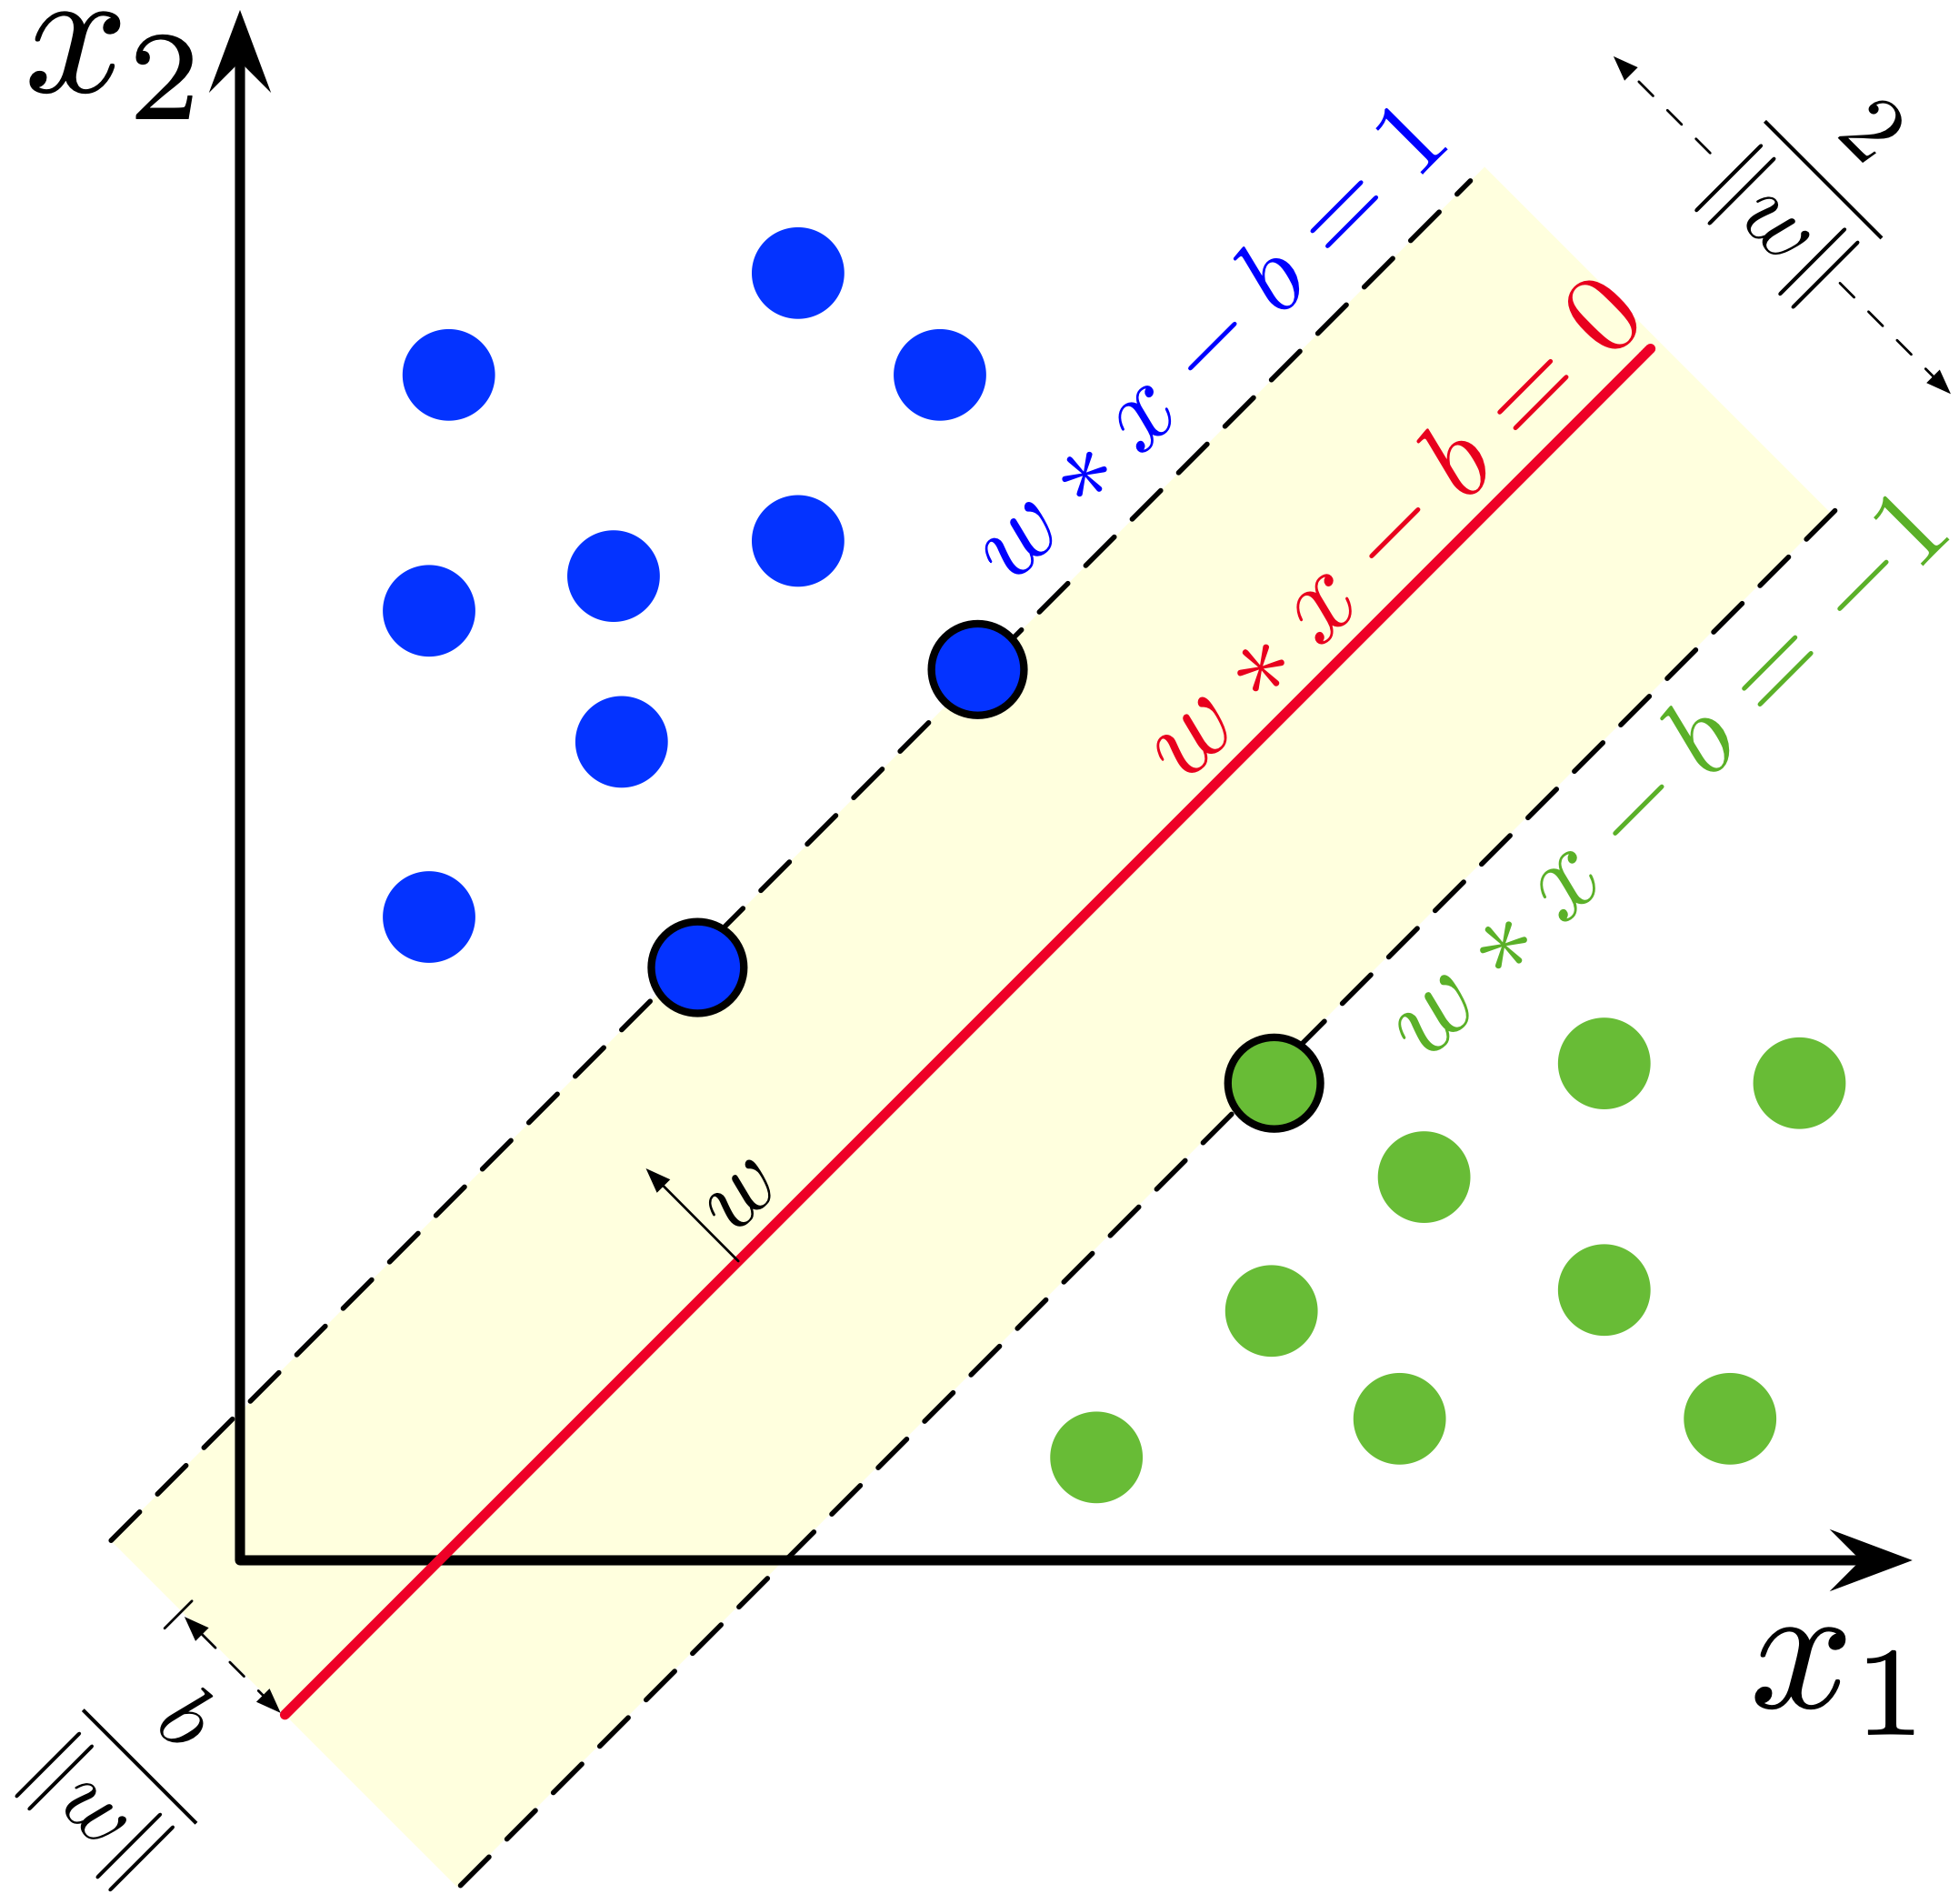
\includegraphics[width=.4\linewidth]{fig/SVM_margin_binary.png}
	\vspace*{2mm}
	\captionfootnotemark{A Hyper-plane and its margins for an SVM to a binary classification problem.}
	\label{simple_svm}
\end{figure}
\footnotetext{Retrieved from: \hyperrefurl{https://en.wikipedia.org/wiki/Support-vector_machine} on April 11, 2021.}

The linear SVM hyper-plane is defined as:

\be
\label{eq:linear_hyperplane}
\textbf{w}^{T}\textbf{x} - b = 0,
\ee

where x is a p-dimensional real vector, w is a weight vector normal to the hyper-plane, and b is a real valued bias parameter. Thus the distance between margins can be computed as $\frac{2}{\norm{\textbf{w}}_{2}}$, and we want to maximize it.

\subsubsection*{\textit{Loss Functions}}

First, let us name the hyper-plane and margins in Figure~\ref{simple_svm} as:

\begin{itemize}
    \item \textbf{hyper-plane:} 
    \be \label{h0_formula} H_{0} = \textbf{w}^{T}\textbf{x} - b = 0 \:,\ee
    \item \textbf{margin for label +1:}
    \be \label{h+1_formula} H_{+1} = \textbf{w}^{T}\textbf{x} - b = +1 \:,\:\text{and}\ee
    \item \textbf{margin for label -1:}
    \be \label{h-1_formula} H_{-1} = \textbf{w}^{T}\textbf{x} - b = -1 \:.\ee
\end{itemize}

Thus, we have the following condition and result relationships for a sample $\textbf{x}^{i}$ p-dimensional real vector with its estimated label $y^{i}$ where $y^{i}$ is either -1 or +1:

\begin{itemize}
    \item if $\textbf{w}^{T}\textbf{x}^{i} - b \geq +1$ and $y^{i} = +1$, then the prediction is correct and the sample belongs to class +1;
    \item else, if $\textbf{w}^{T}\textbf{x}^{i} - b \leq -1$ and $y^{i} = -1$, then the prediction is correct and the sample belongs to class -1;
    \item else, the prediction is incorrect and the sample belongs to opposite of predicted label.
\end{itemize}

When we compound the above conditions, we yield the common condition as:

\begin{equation}
\label{common_loss} 
1 - (\textbf{w}^{T}\textbf{x}^{i} - b)y^{i} \leq 0\:.
\end{equation}

And finally, the margin perception loss function, called as hinge loss, is written as:

\begin{equation}
\label{hinge_loss} 
loss_{hinge}(\textbf{w}, b) = \sum_{i=1}^{n} \max(0, 1 - (\textbf{w}^{T}\textbf{x}^{i} - b)y^{i}).
\end{equation}

Besides, the squared hinge loss is defined as:

\begin{equation}
\label{squared_hinge_loss} 
loss_{squaredHinge}(\textbf{w}, b) = \sum_{i=1}^{n} (\max(0, 1 - (\textbf{w}^{T}\textbf{x}^{i} - b)y^{i}))^{2}.
\end{equation}

The constrained optimization problem of SVM is derived as:

\be
\label{eq:primal_svm}
\min_{w}\ell(\textbf{w})= \min_{w} \frac{\norm{\textbf{w}}_{2}^{2}}{2}\quad \text{such that} \:\:
(\textbf{w}^{T}\textbf{x}^{i} - b)y^{i} - 1 \geq 0 \:, \forall i \in \{1, ..., n\}
\ee

The equation (\ref{eq:primal_svm}) is called as the primal problem.

By using the Lagrange Function with real valued lagrange multipliers $\alpha_{i}$ greater than or equal to 0, the dual problem to solve is constructed as:

\be
\label{eq:dual_svm}
\max_{\alpha}\Lag(\alpha) = \max_{\alpha} \sum_{i=1}^{n}\alpha_{i} - \frac{1}{2}\sum_{i=1}^{n}\sum_{j=1}^{n}\alpha_{i}\alpha_{j}\:y^{i}y^{i}\:{\textbf{x}^{i}}^{T}\textbf{x}^{j}\quad \text{such that} \:\:\sum_{i=1}^{n}\alpha_{i}y^{i} = 0,
\ee

where $x_{i}$ and $y_{i}$ are a p-dimensional real valued feature vector and its label, that is -1 or +1, respectively, $w$ is a weight vector normal to the hyper-plane, b is a real valued bias parameter, and $n$ is the number of samples.

Further details on constraint optimization of SVM, primal and dual problems, and their solutions can be found at  \cite[pg.~13-19]{svm_book}.

\subsubsection*{\textit{Penalty Terms}}
Here $\lambda$ always refers to the regularization parameter during this subsection.
\begin{itemize}
    \item \textbf{L2 Regularizer:} According to \cite[pg.~2054-2059]{svm_penalty}, let first recall the primal form of SVM optimization problem in equation (\ref{eq:primal_svm}). We can modify the problem as:
    \be
    \label{eq:l2_svm_primal}
    \min_{\textbf{w}, b} \Big \{ \sum_{i=1}^{n}[1 - (\textbf{w}^{T}\textbf{x}^{i} - b)y^{i}]_{+} + \lambda \frac{\norm{\textbf{w}}_{2}^{2}}{2} \Big\},
    \ee
    
    where $[1 - (\textbf{w}^{T}\textbf{x}^{i} - b)y^{i}]_{+}$ is the hinge loss term $\max(0, 1 - (\textbf{w}^{T}\textbf{x}^{i} - b)y^{i})$. Yet, the squared hinge loss can be placed as well.
    
    Then, the corresponding dual problem can be obtained as:
    \be
    \label{eq:l2_svm_dual}
    \max_{\alpha} \sum_{i=1}^{n}\alpha_{i} - \frac{1}{2}\sum_{i=1}^{n}\sum_{j=1}^{n}\alpha_{i}\alpha_{j}\:y^{i}y^{i} \big ( \:{\textbf{x}^{i}}^{T}\textbf{x}^{j} + \lambda \delta_{ij} \big ) \quad \text{such that} \:\:\sum_{i=1}^{n}\alpha_{i}y^{i} = 0\:,
    \ee
    where $\alpha$ is the lagrange multiplier given in the equation (\ref{eq:dual_svm}) and $\delta_{ij}$ is the Kronecker’s delta function such that it returns $1$ for $i=j$, and $0$ otherwise.
    
    \item \textbf{L1 Regularizer:}
    As stated in \cite[pg.~2054-2059]{svm_penalty}, L1 regularization is only applicable for the linear SVM problem. The L1 penalized SVM optimization problem is given by the following equation where the $loss(\textbf{w}, b)$ is either hinge or squared hinge loss function:
    \be
    \label{eq:l1_svm_primal}
    \min_{\textbf{w}, b} \sum_{i=1}^{n} loss(\textbf{w}, b) + \lambda  \norm{\textbf{w}}_{1}\:.
    \ee
    
    Then, the corresponding dual problem can be obtained as:
    \be
    \label{eq:l1_svm_dual}
    \max_{\alpha}\Lag(\alpha) \quad  \text{such that} \:\:\sum_{i=1}^{n}\alpha_{i}y^{i} = 0 \:\:\text{and}\:\: 0 \leq \alpha_{i} \leq \frac{1}{\lambda}\:,
    \ee
    where $\Lag$ and $\alpha_{i}$ are lagrange function and lagrange multipliers given in the equation (\ref{eq:dual_svm}).
    
    
\end{itemize}


\subsubsection*{\textit{Kernel Trick}}

Kernel trick is using a feature transformation $\phi$ to map samples into a new space where samples become linearly separable. Then all appearances of samples are replaced with the transformation $\phi$. Now, the kernel function for p-dimensional feature vectors $\textbf{x}_{i}$ and $\textbf{x}_{i}$ is defined as:

\be
\label{eq:kernel_function}
K(\textbf{x}_{i}, \textbf{x}_{j}) = <\phi(\textbf{x}_{i}), \phi(\textbf{x}_{j})> = \phi(\textbf{x}_{i})^{T}\phi(\textbf{x}_{j}).
\ee

This replacement affects to the whole structure of SVM optimization problem.

The most used kernel functions, that are also experienced in this thesis, are:

\begin{itemize}
    \item \textbf{Linear function:}
    \be
    \label{eq:lienar_kernel_function}
    K(\textbf{x}_{i}, \textbf{x}_{j}) = \textbf{x}_{i}^{T}\textbf{x}_{j}.
    \ee
    
    \item \textbf{Gaussian radial basis function (RBF):}
    \be
    \label{eq:rbf_kernel_function}
    K(\textbf{x}_{i}, \textbf{x}_{j}) = \exp(-\gamma \norm{\textbf{x}_{i}-\textbf{x}_{j}}_{2}^{2})\:,
    \ee
    for $\gamma >0$. It is common to choose $\gamma =\frac{1}{2\sigma ^{2}}$ where $\sigma$ represents the standard deviation of original feature map.
    
    \item \textbf{Sigmoid function:}
    \be
    \label{sigmoid_kernel_function}
    K(\textbf{x}_{i}, \textbf{x}_{j}) = \tanh(\alpha \textbf{x}_{i}^{T}\textbf{x}_{j} + c)\:,
    \ee
    for some $\alpha > 0$ and $c < 0$, and $\tanh(.)$ refers the hyperbolic tangent function.

\end{itemize}



\subsection{Logistic Regression (LR)}
Logistic regression (LR) aims to solve binary classification problems. If the problem contains more than 2 classes, the model named as Multinomial LR can be used.
In the logistic model, each sample $\textbf{x} \in \setsymbol{R}^{d}$ has a predicted value $ 0 \leq Pr(\textbf{x}) \leq 1$ referring if the sample belongs to its actual label $y$ or not. If $0.5 < Pr(\textbf{x})$, then the prediction is true. By using the logistic sigmoid function, the model is obtained as:

\be
\label{eq:logistic_p}
Pr(\textbf{x}) = \frac{1}{ 1 + e^{-(\textbf{w}^{T}\textbf{x}+b)} }\:,
\ee

where $\textbf{w} \in \setsymbol{R}^{d}$ is the weight parameter tuning the scaling, and $b \in \setsymbol{R}$ is the bias term tuning the shifting in logistic sigmoid function.

\begin{figure}[h]
	\centering
	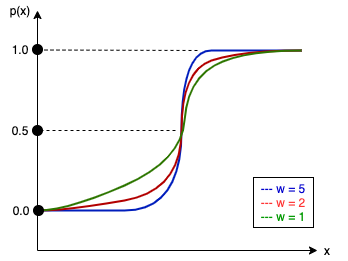
\includegraphics[width=.6\linewidth]{fig/logistic_function.png}
	\vspace*{2mm}
	\caption{Logistic sigmoid function with different scaling w values. }
	\label{logistic_function}
\end{figure}

The sharpness of logistic curve increases with higher $\textbf{w}$ values, and vice versa.

Simply, the hypothesis function can be obtained from sigmoid function as:

\be
\label{eq:logistic_hyptothesis}
\ln \Big (\frac{Pr(\textbf{x})}{1 - Pr(\textbf{x})} \Big ) = \textbf{w}^{T}\textbf{x}+b\:.
\ee

Here, $\frac{Pr(\textbf{x})}{1 - Pr(\textbf{x})}$ is called as odd, and $\log \Big (\frac{Pr(\textbf{x})}{1 - Pr(\textbf{x})} \Big )$ as logit.

For simplicity, let define $z = \textbf{w}^{T}\textbf{x}+b$. Then, we have following constraints:

\begin{itemize}
    \item if $y = 1$, we want $Pr(z) \approx 1$, i.e $z >> 0$, and
    \item if $y = 0$, we want $Pr(z) \approx 0$, i.e $z << 0$.
\end{itemize}

Now, we can construct the log-loss function for a sample pair $(\textbf{x}^{i}, y^{i})$ for $i \in \{1, ..., n\}$ as:

\begin{equation}
\label{log_loss_onesample} 
loss^{i}(\textbf{w}, b) = -y\ln(Pr(z^{i}))  + (1-y)\ln(1-Pr(z^{i})).
\end{equation}

Consequently, the optimization problem is yielded as:

\begin{equation}
\label{lr_optimization} 
\max_{\textbf{w}, b} \ell(\textbf{w}, b) = \max_{\textbf{w}, b} \sum_{i=1}^{n} loss^{i}(\textbf{w}, b).
\end{equation}

\subsubsection*{\textit{Penalty Terms}}
Here $\lambda$ always refers to the regularization parameter during this subsection.

\begin{itemize}
    \item \textbf{L2 Regularizer:}
        \begin{equation}
        \label{lr_l1} 
        \max_{\textbf{w}, b} \ell(\textbf{w}, b) + \lambda \norm{w}_{2}^{2}.
        \end{equation}
    \item \textbf{L1 Regularizer:}
        \begin{equation}
        \label{lr_l1} 
        \max_{\textbf{w}, b} \ell(\textbf{w}, b) + \lambda \norm{w}_{1}.
        \end{equation}
\end{itemize}

\subsubsection*{\textit{Optimizers}}

In this thesis, to solve the optimization problem on LR problem, we use the following the solvers presented by scikit-learn package \cite{scikit-learn} in Python programming language:

\begin{itemize}
    \item Newton’s Method (newton-cg) \cite{lr_newton_cg}, 
    
    \item Limited-Memory Broyden–Fletcher–Goldfarb–Shanno Algorithm \\(lbfgs) \cite{lr_lbfgsb},
    
    \item A Library for Large Linear Classification (liblinear) \cite{lr_liblinear},
    
    \item Stochastic Average Gradient (sag) \cite{lr_sag}, and
    
    \item SAGA \cite{lr_saga}.
\end{itemize}

Different types of optimizers were used for a better approximation to the loss function, and to find the best minimization on this loss function.

Table~\ref{tab:lr_solver_table} shows the solvers eligibility to regularizers.
%% https://stackoverflow.com/questions/38640109/logistic-regression-python-solvers-defintions
\begin{table}[h]
\centering
\caption{Logistic Regression optimization problem solvers.}
\label{tab:lr_solver_table}
\begin{tabular}{|l|c|c|c|}
\hline
\multicolumn{1}{|c|}{\multirow{2}{*}{Solver}} & \multicolumn{3}{c|}{Optimization Problem}                                                                                                                                                                                            \\ \cline{2-4} 
\multicolumn{1}{|c|}{}                        & \multicolumn{1}{l|}{\begin{tabular}[c]{@{}l@{}}No \\ Penalty\end{tabular}} & \multicolumn{1}{l|}{\begin{tabular}[c]{@{}l@{}}L1 \\ Penalty\end{tabular}} & \multicolumn{1}{l|}{\begin{tabular}[c]{@{}l@{}}L2 \\ Penalty\end{tabular}} \\ \hline
newton-cg                                    & X                                                                          &                                                                            & X                                                                          \\ \hline
lbfgs                                         & X                                                                          &                                                                            & X                                                                          \\ \hline
liblinear                                    &                                                                            & X                                                                          & X                                                                          \\ \hline
sag                                         & X                                                                          &                                                                            & X                                                                          \\ \hline
saga                                             & X                                                                          & X                                                                          & X                                                                          \\ \hline
\end{tabular}
\end{table}

\subsection{K-Nearest Neighbor (KNN)}

K-Nearest Neighbor (KNN) algorithm is a classification algorithm developed by Fix, E. and Hodges, L. in 1951 \cite{knn_pdf}. KNN can be used for regression as well; however, at this time the, the output for an object is not a class label, but the property value which is the average of the values of its k nearest neighbors. For both usage cases, KNN is a supervised learning algorithm.

\phantomsection
\subsubsection*{\textit{Algorithm}}

Below, the basic algorithm for KNN is explained for n samples $\textbf{x}^{i} \in \setsymbol{R}^{d}$ and their corresponding class labels $c^{i} \in \{-1, +1\}$. Let the target pair is referred by $(\textbf{x}^{*}, c^{*})$.

\begin{enumerate}
    \item The K nearest neighbors of $\textbf{x}^{*}$ is found with respect to distance between target $\textbf{x}^{*}$ and all other samples. To calculate the distance, different metric functions may be used. The used metrics in this thesis are:
    \begin{itemize}
        \item \textbf{Euclidean Distance:}
        \be
        \label{eucledian_distance}
        d(\textbf{x}^{*}, \textbf{x}^{i}) = \sqrt{\sum_{j=1}^{p} ({\textbf{x}^{*}}_{j} - {\textbf{x}^{i}}_{j})^{2}}\:,
        \ee
        
        \item \textbf{Manhattan Distance:}
        \be
        \label{manhattan_distance}
        d(\textbf{x}^{*}, \textbf{x}^{i}) = \sum_{j=1}^{p} |{\textbf{x}^{*}}_{j} - {\textbf{x}^{i}}_{j}|\:, \text{and}
        \ee
        
        \item \textbf{Chebyshev Distance:}
        \be
        \label{chebyshev_distance}
        d(\textbf{x}^{*}, \textbf{x}^{i}) = \max (|{\textbf{x}^{*}}_{1} - {\textbf{x}^{i}}_{1}|, |{\textbf{x}^{*}}_{2} - {\textbf{x}^{i}}_{2}|, \dots, |{\textbf{x}^{*}}_{p} - {\textbf{x}^{i}}_{p}|)\:.
        \ee
    \end{itemize}
    \item The class label for $\textbf{x}^{*}$ is estimated by majority voting around K nearest neighbors of target sample found in step 1. Majority voting makes its decision by looking for which class label has the majority in appearance around K nearest neighbors. Hence, K is preferred as an odd number. For example, if the K is chosen as 3 and 3 nearest neighbors has class labels as $\{+1, -1, +1\}$, then majority voting predicts the target label as +1 since it appears more than label -1. Besides, it can be considered that all of the voters may not have the same effect. In this scenario, one can use weighted majority voting which allows the closer neighbor in K nears neighbors to have the higher effect. That is, the weight of a voter is the multiplicative inverse of its distance to the target sample. For example, assume that the K is chosen as 3 and 3 nearest neighbors has class labels as $\{+1, -1, +1\}$ with their distances to the target sample as $\{3, 1, 2\}$ respectively. Then the weights of the neighbors are considered as $\{\frac{1}{3}, 1, \frac{1}{2}\}$ or $\{2, 6, 3\}$ respectively. Here, the label -1 has the majority; thus, the target label is predicted as -1.
\end{enumerate}

\begin{figure}[h]
	\centering
	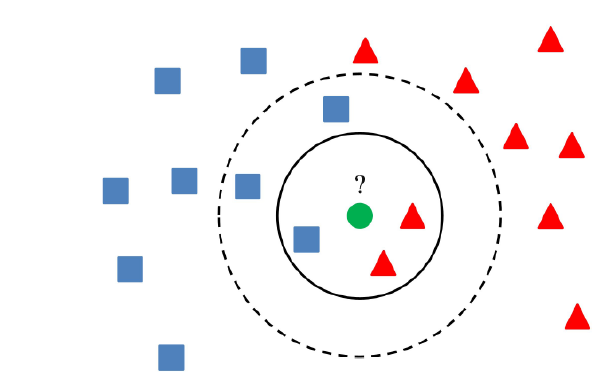
\includegraphics[width=.6\linewidth]{fig/knn_example.png}
	\vspace*{2mm}
	\captionfootnotemark{KNN example illustration to detect the class for the green sample in the middle.}
	\label{knn_example}
\end{figure}
\footnotetext{Retrieved from: \hyperrefurl{https://ai.plainenglish.io/k-nearest-neighbors-from-scratch-633dfbeac740} on April 17, 2021.}

At Figure~\ref{knn_example}, when K = 3, it is labeled as red both by majority voting and weighted majority voting. However, when K = 5, it may change whether to use majority voting or weighted majority voting. It is labeled as blue by majority voting; but, it may be labeled as red by the weighted majority voting.

\subsubsection*{\textit{Finding Neighborhood}}

In this thesis, three algorithms presented by scikit-learn
package \cite{scikit-learn} in Python programming language are used.

%% https://scikit-learn.org/stable/modules/neighbors.html#nearest-neighbor-algorithms
\begin{itemize}
    \item \textbf{Brute Force:} Distances between all pairs of samples are computed. Brute force may be quite efficient for small sized dataset.
    
    \item \textbf{K-Dimensional Tree:} Since brute force becomes inefficient by the increase of dataset size, K-Dimensional (K-D) tree may be used to reduce the required number of computations. If samples $x_{0}$ and $x_{1}$ are very distant, and $x_{1}$ and $x_{2}$ are very close, then we can conclude that $x_{0}$ and $x_{2}$ are very distant too. To create a K-D tree structure, the data space partitioned along the Cartesian axes. Because of the curse of dimensionality, the construction of K-D tree may be inefficient for large dimensions. Further information can be found at \cite{kd_tree}.
    
    \item \textbf{Ball Tree:} Ball tree algorithm was developed to solve the size and dimensionality problems. The data space are partitioned along the Spherical axes to construct the tree structure; hence it is more costly than K-D tree. However the structure itself is more effective, especially in high dimensions. Further information can be found at \cite{ball_tree}.
    
\end{itemize}

\subsection{Linear Discriminant Analysis (LDA)}

The linear discriminant analysis (LDA) is a supervised learning algorithm that is generalized from discriminant analysis developed by Sir Ronald Fisher, who was an statistician, geneticist, and academic, in 1936.

\phantomsection
\subsubsection*{\textit{Derivation}}

A discriminant function $g(\textbf{x})$ from $\setsymbol{R}^{d}$ to $\setsymbol{R}$ is, generally, a monotonically increasing function defining a boundary between two groups or classes. Here $\textbf{x} \in \setsymbol{R}^{d}$ is a sample with $d$ features. $g_{i}(\textbf{x})$ is the probability of x belonging to class $c_{i}$ as given below:

\be
    \label{eq:prob_x_to_ci}
    g_{i}(\textbf{x}) = Pr(c_{i} | \textbf{x}) = \frac{Pr(\textbf{x}|c_{i}) Pr(c_{i})}{Pr(\textbf{x})}, 
\ee

where $Pr(c_{i} | \textbf{x})$ is the likelihood of observing $\textbf{x}$ given class $c_{i}$, $Pr(c_{i})$ is the prior probability of belonging to class $c_{i}$, and $Pr(x)$ is the marginal likelihood of observing $\textbf{x}$. Here, we discard the $Pr(x)$ since observing $\textbf{x}$ is independent of class.

For normal data distribution, we can take the logarithm of $g(\textbf{x})$ since it is monotonically increasing:

\be
\label{eq:log_g}
g_{i}(\textbf{x}) = \ln(Pr(c_{i}|\textbf{x})) = \ln(Pr(\textbf{x}|c_{i})) + \ln(Pr(c_{i}))\:.
\ee

Here, we suppose that the class density $Pr(x|c_{i})$ is normal distribution with mean $\mu_{i}$ and variance $\Sigma_{i}$ where $\Sigma$ describes the covariance matrix considered as $\sigma^{2}I$.

\be
\label{eq:normal_distribution}
Pr(\textbf{x}|c_{i}) = \frac{1}{(2\pi)^{d/2}|\Sigma_{i}|^{1/2}} \exp \Big[ -\frac{1}{2}(\textbf{x} - \mu_{i})^{T}{\Sigma_{i}}^{-1}(\textbf{x} - \mu_{i}) \Big].
\ee

By inserting equation (\ref{eq:normal_distribution}) into equation (\ref{eq:log_g}), we yield:

\be
\label{eq:prior_linear_disc_func}
g_{i}(\textbf{x}) = -\frac{1}{2}(\textbf{x} - \mu_{i})^{T}{\Sigma_{i}}^{-1}(\textbf{x} - \mu_{i}) -\frac{d}{2}\ln(\frac{\pi}{2}) -\frac{1}{2}\ln|\Sigma_{i}| + \ln(Pr(c_{i}))\:.
\ee

Finally, since $\frac{d}{2}\ln(\frac{\pi}{2})$ is constant, we obtain the linear discriminant function for class $i$ as:

\be
\label{eq:linear_disc_func}
g_{i}(\textbf{x}) = -\frac{1}{2}(\textbf{x} - \mu_{i})^{T}{\Sigma_{i}}^{-1}(\textbf{x} - \mu_{i}) -\frac{1}{2}\ln|\Sigma_{i}| + \ln(Pr(c_{i}))\:.
\ee

This linear discriminant function outputs the likelihood of $\textbf{x}$ to be in the class {i}.

There are two presumptive cases on the linear discriminant function. 

\begin{itemize}
    \item \textbf{$\Sigma_{i} = \sigma^{2}I$:} All features have different means, but the same variants.
    \begin{flalign}
        \label{linear_disc_func_case1}
        \nonumber
        &g_{i}(\textbf{x}) = -\frac{1}{2\sigma^{2}}(\textbf{x} - \mu_{i})^{T}(\textbf{x} - \mu_{i}) -\frac{1}{2}\ln(\sigma^{2d}) + \ln(Pr(c_{i}))\:,\\
        \nonumber
        &g_{i}(\textbf{x}) = -\frac{1}{2\sigma^{2}}(\textbf{x} - \mu_{i})^{T}(\textbf{x} - \mu_{i}) + \ln(Pr(c_{i}))\quad \text{since}\:\: \frac{1}{2}\ln(\sigma^{2d})\:\: \text{is constant,}\\
        \nonumber
        &g_{i}(\textbf{x}) = -\frac{1}{2\sigma^{2}} \big ( \textbf{x}^{T}\textbf{x} - \textbf{x}^{T}\mu_{i} - \mu_{i}^{T}\textbf{x} - \mu_{i}^{T}\mu_{i} \big ) + \ln(Pr(c_{i}))\:,\\
        \nonumber
        &g_{i}(\textbf{x}) = -\frac{1}{2\sigma^{2}} \big ( -2\textbf{x}^{T}\mu_{i} - \mu_{i}^{T}\mu_{i} \big ) + \ln(Pr(c_{i}))\quad \text{since}\:\:\textbf{x}^{T}\textbf{x} \:\: \text{is constant and}\:\: \textbf{x}^{T}\mu_{i} = \mu_{i}^{T}\textbf{x}\:,\\
        &g_{i}(\textbf{x}) = \frac{\mu_{i}^{T}}{\sigma^{2}}\textbf{x} + \Big (\ln(Pr(c_{i})) -\frac{\mu_{i}^{T}\mu_{i}}{2\sigma^{2}} \Big ).
    \end{flalign}
    
    It can be seen that, the final discriminant function in equation (\ref{linear_disc_func_case1}) is a linear function.
    
    \item \textbf{$\Sigma_{i} = \Sigma$:} Covariance matrices are all arbitrary, but equal across classes.
    
    \begin{flalign}
        \label{linear_disc_func_case2}
        \nonumber
        &g_{i}(\textbf{x}) = -\frac{1}{2}(\textbf{x} - \mu_{i})^{T}\Sigma^{-1}(\textbf{x} - \mu_{i}) -\frac{1}{2}\ln|\Sigma| + \ln(Pr(c_{i}))\:,\\
        \nonumber
        &g_{i}(\textbf{x}) = -\frac{1}{2}(\textbf{x} - \mu_{i})^{T}\Sigma^{-1}(\textbf{x} - \mu_{i}) + \ln(Pr(c_{i}))\quad \text{since}\:\: \ln|\Sigma|\:\: \text{is constant,}\\
        \nonumber
        &g_{i}(\textbf{x}) = \frac{-1}{2}\big ( \textbf{x}^{T}\Sigma^{-1}\textbf{x} - \mu_{i}\Sigma^{-1}\textbf{x} \textbf{x}^{T}\Sigma^{-1}\mu_{i} + \mu_{i}^{T}\Sigma^{-1}\mu_{i}\big ) + \ln(Pr(c_{i}))\:,\\
        \nonumber
        &g_{i}(\textbf{x}) = \frac{-1}{2}\big( -2\textbf{x}^{T}\Sigma^{-1}\mu_{i} + \mu_{i}^{T}\Sigma^{-1}\mu_{i} \big) + \ln(Pr(c_{i}))\quad \text{since}\:\: \textbf{x}^{T}\Sigma^{-1}\textbf{x}\:\: \text{is constant}\\
        \nonumber
        &\text{and }\:\:\textbf{x}^{T}\Sigma^{-1}\textbf{x} = \mu_{i}\Sigma^{-1}\textbf{x}\:,\\
        &g_{i}(\textbf{x}) = \big( \mu_{i}^{T}\Sigma^{-1} \big) \textbf{x} + \Big(\ln(Pr(c_{i})) -\frac{1}{2}\mu_{i}^{T}\Sigma^{-1}\mu_{i} \Big)\:.
    \end{flalign}
    
    It can be seen that, the final discriminant function in equation (\ref{linear_disc_func_case2}) is a linear function.
    
\end{itemize}

\begin{figure}[h]
	\centering
	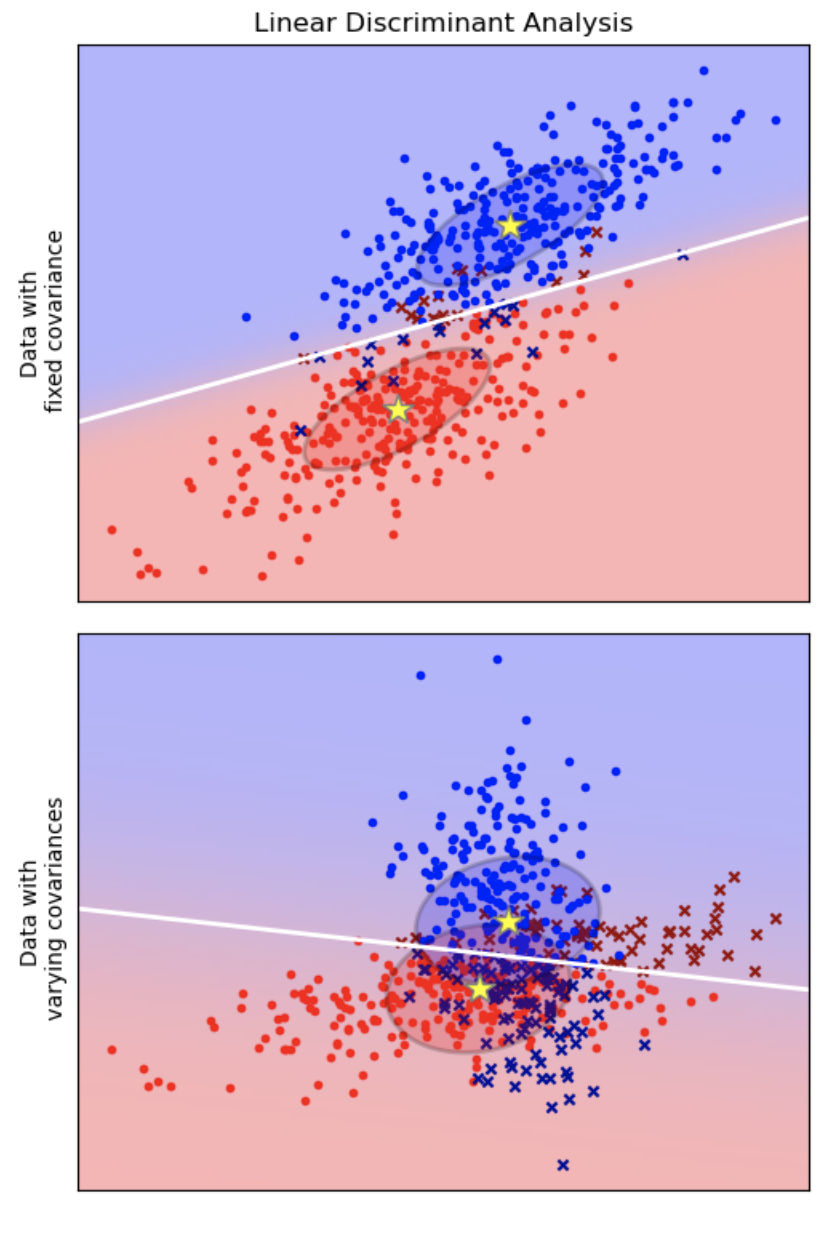
\includegraphics[width=.6\linewidth]{fig/lda.png}
	\captionfootnotemark{LDA process for fixed and varying covariances.}
	\label{lda_example}
\end{figure}
\footnotetext{Retrieved from: \hyperrefurl{https://scikit-learn.org/stable/modules/lda_qda.html} on April 18, 2021.}

\subsubsection*{\textit{Penalty Terms}}
Since high dimensionality may cause LDA not to be optimal and hard to operate over matrices. That is why, a simple modification on covariance matrix is made as \cite{regularized_lda}:

\be
\label{cov_regularization}
\widehat{\Sigma} = \alpha\Sigma + (1-\alpha)I,
\ee

for some real valued $\alpha$ in between the range of $[0, 1]$. We can consider this regularization as what we are used to use in Section~\ref{sec:CH5_regularization}:

\begin{flalign}
    &\widehat{\Sigma} = \lambda\Sigma + I\quad\text{, or}\\
    &\widehat{\Sigma} = \Sigma + \lambda I\:,
\end{flalign}

for positive real valued regularization parameter $\lambda$. Consequently, the regularized LDA is formulated as:

\be
\label{eq:regularized_linear_disc_func}
g_{i}(\textbf{x}) = -\frac{1}{2}(\textbf{x} - \mu_{i})^{T}{\widehat{\Sigma}_{i}}^{-1}(\textbf{x} - \mu_{i}) -\frac{1}{2}\ln|\widehat{\Sigma}_{i}| + \ln(Pr(c_{i}))\:.
\ee

\subsubsection*{\textit{Solvers}}

In this thesis, to solve the LDA functions, we use the solvers presented by scikit-learn
package \cite{scikit-learn} in Python programming language.

Further information about estimators provided by scikit-learn package can be found at \cite{scikit-learn_lda-solvers}.

%% https://scikit-learn.org/stable/modules/lda_qda.html#estimation-algorithms